% \iffalse
\let\negmedspace\undefined
\let\negthickspace\undefined
\documentclass[journal,12pt,twocolumn]{IEEEtran}
\usepackage{cite}
\usepackage{amsmath,amssymb,amsfonts,amsthm}
\usepackage{algorithmic}
\usepackage{graphicx}
\usepackage{textcomp}
\usepackage{xcolor}
\usepackage{txfonts}
\usepackage{listings}
\usepackage{enumitem}
\usepackage{mathtools}
\usepackage{gensymb}
\usepackage{comment}
\usepackage[breaklinks=true]{hyperref}
\usepackage{tkz-euclide} 
\usepackage{listings}
\usepackage{gvv}                                        
\def\inputGnumericTable{}                                
\usepackage[latin1]{inputenc}                            
\usepackage{color}                                       
\usepackage{array}                                       
\usepackage{longtable}                                   
\usepackage{calc}                              
\usepackage{tikz}
\usepackage{multirow}                                    
\usepackage{hhline}                                      
\usepackage{ifthen}                            
\usepackage{caption}
\usepackage{lscape}
\usepackage{amsmath}
\newtheorem{theorem}{Theorem}[section]
\newtheorem{problem}{Problem}
\newtheorem{proposition}{Proposition}[section]
\newtheorem{lemma}{Lemma}[section]
\newtheorem{corollary}[theorem]{Corollary}
\newtheorem{example}{Example}[section]
\newtheorem{definition}[problem]{Definition}
\newcommand{\BEQA}{\begin{eqnarray}}
\newcommand{\EEQA}{\end{eqnarray}}
\newcommand{\define}{\stackrel{\triangle}{=}}
\theoremstyle{remark}
\newtheorem{rem}{Remark}

\begin{document}

\bibliographystyle{IEEEtran}
\vspace{3cm}

\title{NCERT Math 11.9.2 Q8}
\author{EE23BTECH11009 - AROSHISH PRADHAN$^{*}$% <-this % stops a space
}
\maketitle
\newpage
\bigskip
\textbf{Question:} If the sum of $n$ terms of an AP is $(pn + qn^2)$, where $p$ and $q$ are constants, find the common difference.\\

\solution
\begin{table}[!h]
    \centering
    \begin{table}[!h]
    \centering
    \begin{tabular}{|c|c|c|}
    \hline
       \textbf{Symbol}  & \textbf{Value} &  \textbf{Description}\\
    \hline
       $V_{in}$  &  &  Input Voltage\\
    \hline
        $V_{out}$ & & Output Voltage\\
    \hline
        $f$ & $1000Hz$ & Input Wave Frequency\\
    \hline
        $T$ & $\dfrac{1}{f} = 10^{-3} s$ & Input Wave Time Period\\
    \hline
        \multirow{4}{*}{$R$} & (a) $0.5k\Omega$ & \multirow{4}{*}{Resistance}\\
        \cline{2-2}
        & (b) $5k\Omega$ &\\
        \cline{2-2}
        & (c) $0.5k\Omega$ &\\
        \cline{2-2}
        & (d) $5k\Omega$ &\\
    \hline
        \multirow{4}{*}{$C$} & (a) $0.1\mu F$ & \multirow{4}{*}{Capacitance}\\
        \cline{2-2}
        & (b) $1\mu F$ &\\
        \cline{2-2}
        & (c) $0.1\mu F$ &\\
        \cline{2-2}
        & (d) $1\mu F$ &\\
    \hline
        $\tau$ & $RC$ & Time Constant\\
    \hline
    \end{tabular}
    \caption{Given Parameters}
    \label{tab:1_gate.23.ph.37}
\end{table}

    \caption{Given Parameters}
    \label{tab:1}
\end{table}

Sum of $n$ terms, as a discrete signal:
\begin{equation}
    s(n) = (pn + qn^2)u(n)
\end{equation}

Taking the $Z$-Transform,
\begin{align}
    s(n) &\overset{z}{\longleftrightarrow} S(z)\\
    \implies S(z) &= \sum_{n = - \infty}^{\infty}s(n)z^{-n}\\
    &= \sum_{n = - \infty}^{\infty}(pn + qn^2)u(n)z^{-n}\\
    &= p\sum_{n = -\infty}^{\infty}nu(n)z^{-n} + q\sum_{n = -\infty}^{\infty}n^2u(n)z^{-n}\\
    &= p\left(\dfrac{z^{-1}}{(1-z^{-1})^2}\right) + q\left(\dfrac{z^{-1}(1 + z^{-1}).}{(1-z^{-1})^3}\right)
\end{align}

where $\{z\in \mathbb{C}: \abs{z} > 1\}$

Now, 
\begin{align}
    s(n) &= x(n) \ast u(n)\\
    \implies S(z) &= X(z)U(z)\\
    \implies X(z) &= \dfrac{S(z)}{U(z)}\label{eq:9}
\end{align}

where,
\begin{align}
    U(z) &= \mathcal{Z}(u(n))\\
    &= \dfrac{1}{1 - z^{-1}}\label{eq:11}
\end{align}

for $\{z\in \mathbb{C}: \abs{z} > 1\}$

Using \eqref{eq:11} in \eqref{eq:9},
\begin{align}
    X(z) &= p\left(\dfrac{z^{-1}}{(1-z^{-1})}\right) + q\left(\dfrac{z^{-1}(1 + z^{-1})}{(1-z^{-1})^2}\right)
\end{align}

Simplifying using partial fractions, we get:
\begin{align}
    X(z) &= (q-p) + \dfrac{p-3q}{1-z^{-1}} + \dfrac{2q}{(1-z^{-1})^2}\\
    &= (q - p) + \dfrac{(p-q)}{1-z^{-1}} + \dfrac{2qz^{-1}}{(1-z^{-1})^2}
\end{align}

Taking the inverse Z-Transform,
\begin{align}
    x(n) = (q-p)\delta(n) + (p-q)u(n) + 2qnu(n)\label{eq:15}
\end{align}
\\
To simplify, use $n=0$:
\begin{equation}
    s(0) = x(0) = 0
\end{equation}
\begin{align}
    &\implies (q-p)\delta(0) + (p-q)u(0) + 2qnu(0) = 0\\
    &\implies p = q
\end{align}

because $\delta(0) \rightarrow \infty$

$\therefore$ rewriting \eqref{eq:15}:
\begin{equation}
    x(n) = 2qnu(n)
\end{equation}

Common difference is given by:
\begin{align}
    d &= x(n+1) - x(n)\\
    &= 2q(n+1)u(n+1) - 2qnu(n)\\
    &= 2q
\end{align}

\begin{figure}[!h]
    \centering
    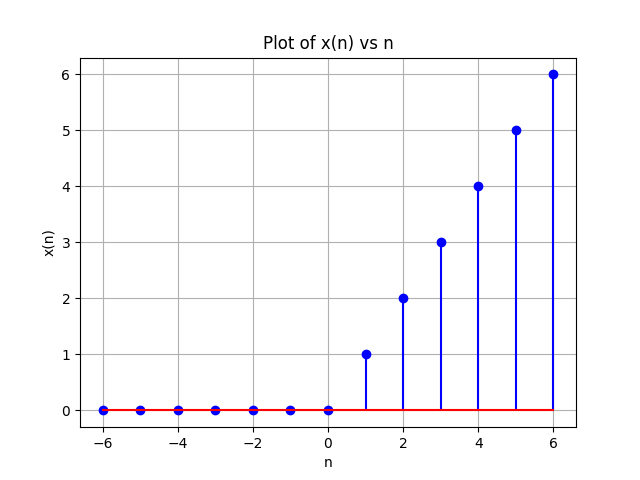
\includegraphics[width = \columnwidth]{figs/x_plot.png}
    \caption{Plot of x(n) vs n}
    \label{fig:1}
\end{figure}
\end{document}
